\documentclass[conference,a4paper]{IEEEtran}

\usepackage{amsmath,amssymb,amsfonts}
\usepackage{graphicx}
\usepackage{textcomp}
\usepackage{xcolor}
\usepackage{booktabs}
\usepackage{array}
\usepackage{listings}
\usepackage{url}
\usepackage{hyperref}
\usepackage{cite}
\usepackage{tikz}
\usetikzlibrary{arrows.meta,positioning}

\lstset{
	basicstyle=\ttfamily\footnotesize,
	keywordstyle=\color{blue}\bfseries,
	commentstyle=\color{gray}\itshape,
	stringstyle=\color{red},
	numbers=left,
	numberstyle=\tiny\color{gray},
	numbersep=5pt,
	frame=single,
	breaklines=true,
	captionpos=b,
	tabsize=4
}

\begin{document}

\title{Performance, Resource Utilization, and Cost Analysis of Web Applications: Virtual Machines vs.\ Docker Containers\\
	{\footnotesize SEN421 --- Cloud Architecture and Services, Course Project, Fall 2026\\
		Istanbul Ayd\i n University}
}

\author{\IEEEauthorblockN{Emre Avcı}
	\IEEEauthorblockA{\textit{Department of Software Engineering}\\
		\textit{Istanbul Ayd\i n University}\\
		Istanbul, Turkey \\
		Student ID: B2105.090126 \\
		emreavci3@stu.aydin.edu.tr}
}

\maketitle

\begin{abstract}
This paper compares a virtual machine and a Docker container hosting the same web API for SEN421 Topic 2 Part A. The question is how much faster a containerized API starts and responds under the same load, and what that speed costs in resources and isolation. The service has a health check, a CPU bound hash route, and a fixed payload route. Both local platforms were capped at two virtual CPUs and two gigabytes of memory. k6 used fifty virtual users for thirty seconds, three times, with fifteen seconds idle between runs. Container median latency was 224.121 milliseconds, sample standard deviation 75.998. The QEMU guest on WHPX had a median of 214.347 milliseconds, sample standard deviation 70.009. Throughput was 174.925 requests per second for the container and 157.792 for the guest. Ready time was 1.450 seconds against 47.660 seconds. Image content was 49.701 mebibytes. The guest disk file was 2.792 gigabytes. The guest failed about six percent of requests. A Frankfurt list price for 730 hours and 196.608 gigabytes of payload traffic is 28.36 USD for one t3.micro with 20 gigabytes of gp3, and 28.06 USD for a Fargate task of 0.25 vCPU and 0.5 GB. No AWS resource was created, so the experiment cost nothing. The container is faster to start, smaller, and slightly faster in throughput. Median latency does not show a shared kernel win, because VirtualBox could not use hardware virtualization and Docker Desktop does not share the Windows kernel.
\end{abstract}

\begin{IEEEkeywords}
	cloud computing, virtualization, Docker containers, performance benchmarking, shared responsibility
\end{IEEEkeywords}

\section{Introduction}
\label{sec:introduction}

A small web API can run in a guest operating system under a hypervisor or in a container that shares the host kernel. The choice changes startup time, the bytes that must be stored, the failure domain, and the monthly bill. An organization that picks the faster option without measuring isolation can move a kernel bug from one service into every neighbor on the host.

The question of this project is: how much faster does a containerized web API start and respond compared with a virtual machine under identical load, and what are the trade-offs in resource overhead and isolation? Topic 2 Part A answers that question by running one FastAPI service in two local environments, applying the same k6 load, and projecting a 730 hour AWS bill. The local comparison is a Docker container against a QEMU guest. The cost comparison is one EC2 \texttt{t3.micro} against one ECS on Fargate task. No autoscaling is measured.

The rest of the paper defines the two execution models, describes the system and the legal boundary, states the test parameters, reports the measured numbers and the price-list bill, and discusses why the median latency does not follow the startup result.

\section{Background and Related Work}
\label{sec:related_work}

NIST defines cloud computing as a model for ubiquitous, convenient, on-demand network access to a shared pool of configurable resources that can be provisioned and released with little management effort~\cite{b1}. The definition lists five essential characteristics, including resource pooling and rapid elasticity, and three service models. Infrastructure as a service leaves the guest operating system to the customer. A container platform moves the host kernel to the provider and leaves the image contents to the customer. That split is the shared-responsibility difference measured indirectly by this project: the same application bytes sit on different amounts of platform code.

West discusses hypervisors and virtualization boundaries in enterprise cloud infrastructure~\cite{b2}. In this study, we operationalize these principles by evaluating Type-2 hypervisor behavior against containerized isolation as documented by Oracle and Docker~\cite{b3}, \cite{b4}. Oracle VM VirtualBox is a type-2 hypervisor: it runs on an installed host operating system, whereas a type-1 hypervisor runs on the hardware~\cite{b3}. A type-2 guest has its own kernel. Docker's security model starts from the opposite arrangement. The Docker documentation names the kernel, and the kernel's namespaces and cgroups, as the isolation mechanism~\cite{b4}. A container has its own process, network, mount, and user view, plus a resource ceiling, but it does not have a private kernel. A kernel fault is therefore a host fault. The virtual machine pays for a second kernel with disk size and boot time, and it keeps that fault inside the guest.

k6 is the load generator specified for the repeated runs~\cite{b5}. Prices are taken from the AWS price list for EC2, ECS, and data transfer, not from a calculator screenshot~\cite{b6}.

\section{System Design}
\label{sec:design}

\subsection{Architecture}

Fig.~\ref{fig:architecture} shows the measurement path. The client is k6 on the Windows host. It calls one target at a time on \texttt{127.0.0.1:8000}. The application is the same three routes in both targets. \texttt{GET /health} returns the fixed body \texttt{\{ "status": "ok" \}}. \texttt{GET /compute} runs 50{,}000 SHA-256 rounds on every request and returns the iteration count and the digest. \texttt{GET /payload} returns a JSON object of exactly 65{,}536 bytes, built once at process start. Two uvicorn workers listen on port 8000. OpenAPI is disabled. There is no database and no secret.

\begin{figure}[htbp]
	\centering
	\resizebox{\columnwidth}{!}{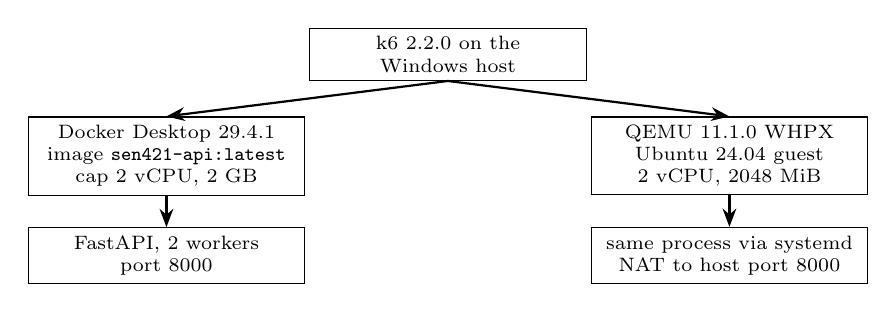
\begin{tikzpicture}[
		font=\scriptsize,
		box/.style={draw, align=center, inner sep=3pt, text width=3.3cm},
		arr/.style={-{Stealth}, thick}
	]
	\node[box] (k6) {k6 2.2.0 on the Windows host};
	\node[box, below left=0.45cm and 0.05cm of k6] (doc) {Docker Desktop 29.4.1\\image \texttt{sen421-api:latest}\\cap 2 vCPU, 2 GB};
	\node[box, below right=0.45cm and 0.05cm of k6] (vm) {QEMU 11.1.0 WHPX\\Ubuntu 24.04 guest\\2 vCPU, 2048 MiB};
	\node[box, below=0.4cm of doc] (a1) {FastAPI, 2 workers\\port 8000};
	\node[box, below=0.4cm of vm] (a2) {same process via systemd\\NAT to host port 8000};
	\draw[arr] (k6.south) -- (doc.north);
	\draw[arr] (k6.south) -- (vm.north);
	\draw[arr] (doc) -- (a1);
	\draw[arr] (vm) -- (a2);
	\end{tikzpicture}}
	\caption{Request path. The two lower branches are alternatives. Only one listener owns host port 8000 during a run.}
	\label{fig:architecture}
\end{figure}

The container target uses Docker Compose. The image is built from \texttt{python:3.12-slim}, runs as \texttt{nobody}, and is limited to 2.0 CPUs, 2~GB of memory, and 2~GB of memory plus swap. The guest target is an Ubuntu 24.04 disk, originally created for VirtualBox, booted with QEMU. The guest address is \texttt{10.0.2.15}. The host reaches it through user-mode NAT. systemd unit \texttt{webapi.service} starts the same uvicorn command.

\subsection{Alternatives Compared}

The performance pair is the local container and the local guest. The cost pair is a projection, because no AWS account resources were created. EC2 is one shared-tenancy Linux \texttt{t3.micro} in \texttt{eu-central-1} with a 20~GB gp3 volume, on demand, for 730 hours, with no load balancer and no Elastic IP. Fargate is one Linux/x86 task at 0.25 vCPU and 0.5~GB of memory for the same 730 hours, again with no load balancer. These cloud shapes are not equal to each other, and neither matches the local cap of 2 vCPU and 2~GB. \texttt{t3.micro} provides 2 vCPU and 1~GiB. The Fargate row is the profile required for this cost model. Fargate also cannot be purchased as 2 vCPU with only 1~GiB.

\subsection{Requirements and Responsibilities}

The design has to serve the three routes, stay inside the CPU and memory caps, and use synthetic data only. Personal data was not collected and was not uploaded.

On the local machine the student is responsible for the host, the hypervisor or the Docker engine, the guest or the image, the application, and the network exposure, which was loopback and NAT. On EC2, AWS is responsible for the facilities, the hardware, and the hypervisor. The customer is responsible for the guest operating system, the application, security groups, and data. On Fargate, AWS is also responsible for the host kernel. The customer remains responsible for the image contents, the task definition, IAM, the network, and the data. If this API later carried personal data, the customer would be the KVKK controller and AWS the processor. \texttt{eu-central-1} is outside Turkey, so KVKK article 9 would govern the transfer. The local runs keep the bytes in Turkey. This paper is not a legal opinion.

\section{Methodology}
\label{sec:methodology}

\subsection{Environment}

Table~\ref{tab:environment} records the parameters needed to repeat the runs. The host operating system is Windows. Docker Desktop on that host runs containers inside a utility virtual machine, so the container numbers are not a native shared-kernel result. VirtualBox 7.2.22 was installed and the guest reached a running state, then fell back to NEM because VT-x was not available and stopped at the initramfs line ``Begin: loading essential drivers.'' The measured guest is therefore QEMU 11.1.0 with \texttt{-accel whpx,kernel-irqchip=off}, using the same VMDK, with 2 vCPU and 2048~MiB.

\begin{table}[htbp]
	\caption{Experimental Environment}
	\label{tab:environment}
	\begin{center}
		\footnotesize
		\begin{tabular}{|p{0.42\linewidth}|p{0.48\linewidth}|}
			\hline
			\textbf{Property} & \textbf{Value} \\
			\hline
			Provider and region & Local Windows host. Cost model: AWS \texttt{eu-central-1} \\
			\hline
			Machine size(s) & Local: 2 vCPU, 2~GB. EC2: \texttt{t3.micro}. Fargate: 0.25 vCPU, 0.5~GB \\
			\hline
			Operating system & Ubuntu 24.04 guest. Container base \texttt{python:3.12-slim} \\
			\hline
			Application & FastAPI 0.156.1, uvicorn 0.54.0, 2 workers, 3 routes \\
			\hline
			Load test tool & k6 2.2.0, 50 virtual users, \texttt{/compute} and \texttt{/payload} \\
			\hline
			Test duration & 30 seconds per run \\
			\hline
			Repetitions & 3 runs, 15 seconds idle between runs \\
			\hline
		\end{tabular}
	\end{center}
\end{table}

\subsection{Measurements}

Each run records the mean, median, and 95th percentile of \texttt{http\_req\_duration} in milliseconds, the request rate, and, for the guest runs, the failed-request percentage. The three Docker summaries were written before the failed-request field existed, so that cell is empty. Image size is \texttt{docker image inspect} field \texttt{Size}, 52{,}115{,}316 bytes (49.701~MiB). The \texttt{docker images} column showed 208~MB for the same image; both numbers are kept. Guest disk size is the VMDK file length after the boots, 2{,}792{,}423{,}424 bytes (2.792~GB). Virtual size remained 64~GiB. Container ready time is the interval from \texttt{docker start} after \texttt{docker stop} until \texttt{/health} returns 200. Guest ready time is the interval from the QEMU process start until the same request returns 200. Sample standard deviation uses divisor \(n-1=2\).

Thresholds were an HTTP 200 rate above 0.99 and a 95th percentile under 500~ms. A run that missed a threshold was saved. It was not deleted and it was not replaced.

\subsection{Cost Model}

The projection uses the public AWS price list, accessed 21 October 2026, currency USD, 730 hours, Linux, shared tenancy, on demand~\cite{b6}. The outbound model counts only \texttt{/payload}: \(65536 \times 3{,}000{,}000 = 196{,}608{,}000{,}000\) bytes = 196.608~GB, from an assumption of 100{,}000 requests per day. Health and compute responses are not in that line. The 100~GB allowance inside the phrase ``beyond the global free tier'' is not subtracted from the headline. No Reserved, Spot, public IPv4, Elastic IP, load balancer, or registry line is included.

\subsection{Reproducibility}

The runner is Listing~\ref{lst:runs} in the Appendix. k6 reads \texttt{BASE\_URL}, default \texttt{http://127.0.0.1:8000}, alternates \texttt{/compute} and \texttt{/payload} by iteration, and writes \texttt{results\_runN.json}. Repository and configuration artifacts are hosted at: \url{https://github.com/Emre1071/sen421-cloud-vm-vs-docker}. AI-assisted tools (Cursor IDE / LLM) were utilized for drafting boilerplate configurations, test harnesses, and LaTeX structural formatting. All test runs, measurements, data analyses, and text syntheses were executed, verified, and finalized by the student.

\section{Results}
\label{sec:results}

\subsection{Performance Results}

Table~\ref{tab:results} is the mean of three runs plus or minus the sample standard deviation. The container median values were 255.423, 279.468, and 137.472~ms. The guest median values were 268.268, 135.227, and 239.547~ms. Container 95th percentiles were 465.741, 480.823, and 809.605~ms, so run 3 missed only the latency threshold. Guest 95th percentiles were 760.030, 786.166, and 658.733~ms. Guest failure rates were 6.471, 6.796, and 4.664 percent. All three guest runs missed both thresholds. The first seconds of guest run 1 included connection-refused warnings. Docker idle memory was 93.08~MiB. Under load the sample peak was 201.52 percent CPU and 99.54~MiB, with a sample mean memory of 97.85~MiB. Fig.~\ref{fig:results} shows the ready-time gap that the latency columns hide.

\begin{table}[htbp]
	\caption{Measured Comparison (mean \(\pm\) sample standard deviation, \(n=3\))}
	\label{tab:results}
	\begin{center}
		\scriptsize
		\begin{tabular}{|l|c|c|}
			\hline
			\textbf{Metric} & \textbf{Docker} & \textbf{QEMU/WHPX} \\
			\hline
			Median (ms) & 224.121 \(\pm\) 75.998 & 214.347 \(\pm\) 70.009 \\
			\hline
			p95 (ms) & 585.389 \(\pm\) 194.322 & 734.976 \(\pm\) 67.310 \\
			\hline
			Req/s & 174.925 \(\pm\) 8.026 & 157.792 \(\pm\) 6.847 \\
			\hline
			Image or disk & 49.701 MiB & 2.792 GB file \\
			\hline
			Boot or ready (s) & 1.450 \(\pm\) 0.221 & 47.660 \(\pm\) 6.244 \\
			\hline
		\end{tabular}
	\end{center}
\end{table}

\begin{figure}[htbp]
	\centering
	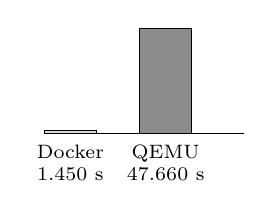
\begin{tikzpicture}
		\begin{scope}[x=0.55cm,y=0.028cm]
			\draw[fill=black!15] (0,0) rectangle (1.2,1.450);
			\draw[fill=black!45] (2.2,0) rectangle (3.4,47.660);
			\draw (0,0) -- (4.6,0);
			\node[anchor=north, font=\scriptsize, align=center] at (0.6,-1) {Docker\\1.450 s};
			\node[anchor=north, font=\scriptsize, align=center] at (2.8,-1) {QEMU\\47.660 s};
		\end{scope}
	\end{tikzpicture}
	\caption{Mean time until \texttt{/health} returned 200. The vertical axis is seconds.}
	\label{fig:results}
\end{figure}

\subsection{Cost Results}

Table~\ref{tab:cost} is list price. EC2 compute is \(0.012 \times 730 = 8.76\) USD (Linux \texttt{t3.micro} instance hour, effective 1 October 2026). gp3 storage is \(0.0952 \times 20 = 1.904\) USD per month (effective 1 October 2026). Fargate compute is \(0.25 \times 0.04656 \times 730 + 0.5 \times 0.00511 \times 730 = 8.4972 + 1.86515 = 10.36235\) USD (vCPU and memory hours, effective 1 October 2026). The task requests no ephemeral storage above the 20~GiB minimum documented for Fargate platform 1.4.0 (\url{https://docs.aws.amazon.com/AmazonECS/latest/developerguide/fargate-task-storage.html}, accessed 21 October 2026), so the Fargate storage line is 0. Data transfer out from EU (Frankfurt) to the internet is 0.090 USD per GB for the first 10~TB beyond the global free tier (effective 1 June 2026). Both rows use \(196.608 \times 0.090 = 17.69472\) USD. Managed services are zero because no load balancer and no registry were priced. The experiment created no cloud resources, so the actual spend is 0 USD.

If the 100~GB allowance were applied, the billable transfer would be 96.608~GB, or 8.69472 USD, and each total would fall by 9.00 USD. That allowance is a note, not the comparison.

\begin{table}[htbp]
	\caption{Monthly List-Price Breakdown, \texttt{eu-central-1}, 730 hours (USD)}
	\label{tab:cost}
	\begin{center}
		\footnotesize
		\begin{tabular}{|l|c|c|}
			\hline
			\textbf{Cost item} & \textbf{EC2 t3.micro} & \textbf{Fargate 0.25/0.5} \\
			\hline
			Compute & 8.76000 & 10.36235 \\
			\hline
			Storage & 1.90400 & 0.00000 \\
			\hline
			Data transfer out & 17.69472 & 17.69472 \\
			\hline
			Managed services & 0.00000 & 0.00000 \\
			\hline
			\textbf{Total (USD)} & \textbf{28.35872} & \textbf{28.05707} \\
			\hline
		\end{tabular}
	\end{center}
\end{table}

\subsection{Comparison of Alternatives}

On the measurements that match the question's ``how much faster,'' the container is faster to become ready by about 46 seconds, and it serves about 17 more requests per second. It is not faster in the median: the guest median is 9.774~ms lower, and both medians have a standard deviation near 70~ms, so that gap is smaller than the spread. The guest is worse at the tail, and it drops about six percent of requests. The container artifact is about 56 times smaller than the guest disk file. The projected bills differ by 0.30 USD, on shapes that do not provide the same CPU or memory.

\section{Discussion}
\label{sec:discussion}

The useful contrast is between latency and resources. The guest, given a private kernel and 2048~MiB, did not produce a clearly better median, and it produced a worse tail, a lower rate, and request loss. The container peak memory sample stayed under 100~MiB while the guest was allocated 2~GB before the application started. Most of the virtual machine's resource cost is the platform, not the request.

Hypervisor overhead shows up in the ready time, not in the 30 second median. A second kernel, an initramfs, and a systemd boot cost 47.660 seconds. Starting an already built container cost 1.450 seconds. That ratio matters when a new copy must appear under load. It does not, by itself, make the steady-state response faster. The guest's NAT path and the container's path through Docker Desktop are both part of the result. They were not removed.

The VirtualBox run is not a completed type-2 measurement. VT-x was unavailable, the hypervisor fell back to NEM, and the guest did not pass the early boot line. WHPX with \texttt{kernel-irqchip=off} booted the same disk and is still a hosted hypervisor, but it is a different product from the VirtualBox configuration in the setup scripts. Docker Desktop is also a virtual machine under Windows. A claim that these numbers isolate cgroups against a type-2 hypervisor requires a later run on one Ubuntu host with Docker Engine and VirtualBox, with VT-x enabled. Until that host exists, the startup and size gaps are real on this machine, and the shared-kernel explanation is not yet isolated.

At production scale several locks break. A \texttt{t3.micro} uses CPU credits, which this 30 second local test does not reproduce. The Fargate price is for a quarter of a vCPU and half a gigabyte, so it is not the cost of the measured 2 vCPU and 2~GB cap. A single region, a synthetic body, and three short runs do not describe a daily traffic curve. The 95th percentile missed the 500~ms bar on both sides, so the acceptance thresholds were not met. Outbound transfer dominates both bills; a payload smaller than 64~KB would shrink the line that is currently larger than compute.

AWS protects the building and, on Fargate, the host kernel. The student still protects the image, the dependency pins, the decision to run as \texttt{nobody}, and the choice not to publish the API. Isolation remains the reason to keep a virtual machine when a kernel bug must not cross a tenant boundary, even if the container is smaller and quicker to start. Personal data would add a residency cost that neither latency table contains: Frankfurt is a cross-border location under KVKK, and the local disk is not.

\section{Conclusion and Future Work}
\label{sec:conclusion}

The container became ready in 1.450 seconds against 47.660 seconds, stored 49.701~MiB against a 2.792~GB disk file, and served 174.925 requests per second against 157.792. The median latencies were 224.121 and 214.347 milliseconds. The guest failed 5.977 percent of requests. The 730 hour list prices were 28.36 USD and 28.06 USD. For this stateless API the container is the better default on startup, size, and throughput, provided a shared kernel is acceptable. The virtual machine remains the choice when the failure domain must include the kernel. The bill does not decide the question, because the priced shapes are smaller than the measured caps and the transfer line is common to both.

With more time the next measurement is a native Ubuntu host with VT-x, VirtualBox, and Docker Engine on the same kernel, repeating the three runs until both thresholds hold. After that, the same image should be scheduled by Kubernetes, so the startup advantage can be checked when more than one replica is created. The price model should then be rebuilt for equal CPU and memory, including any public IPv4 charge the platform adds.

\section*{AI Tool Use and Originality Declaration}
\label{sec:ai_declaration}

AI-assisted tools, specifically Cursor IDE (Claude/GPT engine), were used only for limited support: prompt-based formulation, locating documentation, boilerplate configuration, IEEE formatting, and draft structure. The project idea is the course assignment. Experiments were run locally by the student. Prices were taken from the public AWS price list accessed 21 October 2026. The analysis, critique, and final wording were reviewed and finalized by the student, who accepts full responsibility for the accuracy, originality, reproducibility, and integrity of the submitted work. Table~\ref{tab:ai_use} records that use. The assistant is not an author and is not a source of facts.

\begin{table}[htbp]
	\caption{AI Use Disclosure Summary}
	\label{tab:ai_use}
	\centering
	\footnotesize
	\begin{tabular}{|p{0.32\linewidth}|c|p{0.42\linewidth}|}
		\hline
		\textbf{Project Stage} & \textbf{Level} & \textbf{Brief Description} \\
		\hline
		Topic and question & 1 & Course assignment topic; formulation assisted by prompts. \\
		\hline
		Literature and documentation search & 2 & Assisted in locating NIST, course text, and vendor documentation. \\
		\hline
		Design, deployment, and configuration & 2 & Assisted in drafting boilerplate configs and scripts; verified and run locally by the student. \\
		\hline
		Measurement, cost analysis, and modeling & 2 & Runs executed locally; cost formulas derived from public AWS rates. \\
		\hline
		Writing, editing, and LaTeX formatting & 3 & Assisted with IEEE template formatting, structural styling, and syntax polishing. \\
		\hline
		Interpretation, discussion, and conclusion & 2 & Draft structure assistance; final analysis, critique, and synthesis reviewed and finalized by the student. \\
		\hline
	\end{tabular}
\end{table}

\begin{thebibliography}{00}

	\bibitem{b1} P.~Mell and T.~Grance, ``The NIST definition of cloud computing,'' National Institute of Standards and Technology, Gaithersburg, MD, USA, NIST Special Publication 800-145, 2011.

	\bibitem{b2} J.~West, \textit{CompTIA Cloud+ Guide to Cloud Computing}, 2nd~ed. Boston, MA, USA: Cengage, 2024.

	\bibitem{b3} Oracle, ``Oracle VM VirtualBox User Manual, Chapter 1,'' Oracle VM VirtualBox documentation. [Online]. Available: \url{https://www.virtualbox.org/manual/ch01.html}. [Accessed: 21 October 2026].

	\bibitem{b4} Docker Inc., ``Docker security,'' Docker Documentation. [Online]. Available: \url{https://docs.docker.com/engine/security/}. [Accessed: 21 October 2026].

	\bibitem{b5} Grafana Labs, ``k6 documentation,'' Grafana Labs. [Online]. Available: \url{https://grafana.com/docs/k6/latest/}. [Accessed: 21 October 2026].

	\bibitem{b6} Amazon Web Services, ``AWS Price List: Amazon EC2, Amazon ECS, and AWS Data Transfer, eu-central-1,'' AWS Price List API. [Online]. Available: \url{https://pricing.us-east-1.amazonaws.com/offers/v1.0/aws/AmazonEC2/current/eu-central-1/index.csv}, \url{https://pricing.us-east-1.amazonaws.com/offers/v1.0/aws/AmazonECS/current/eu-central-1/index.csv}, \url{https://pricing.us-east-1.amazonaws.com/offers/v1.0/aws/AWSDataTransfer/current/eu-central-1/index.csv}. [Accessed: 21 October 2026].

\end{thebibliography}

\appendix

\section{Repeated Load Test}
\label{app:code}

Repository and configuration artifacts are hosted at: \url{https://github.com/Emre1071/sen421-cloud-vm-vs-docker}. The runner below is \texttt{load-tests/run\_benchmarks.ps1}. It calls \texttt{load-tests/test-script.js}, which sets 50 virtual users, a 30 second duration, alternating \texttt{/compute} and \texttt{/payload}, and the two thresholds. Each non-zero k6 exit still leaves the JSON in place; the script then returns exit code 1.

\begin{lstlisting}[caption={Repeated k6 runs used for both targets}, label={lst:runs}]
for ($run = 1; $run -le 3; $run++) {
    $env:RESULT_PATH = "$relative/results_run$run.json"
    & k6 run (Join-Path $Root "test-script.js")
    if ($LASTEXITCODE -ne 0) { $failed = $true }
    if ($run -lt 3) { Start-Sleep -Seconds 15 }
}
\end{lstlisting}

\end{document}
